\documentclass[]{report}
\usepackage{listings}
\usepackage{color}
\usepackage{tikz}
\usetikzlibrary{shapes.geometric, arrows}

\definecolor{mygreen}{rgb}{0,0.6,0}
\definecolor{mygray}{rgb}{0.5,0.5,0.5}
\definecolor{mymauve}{rgb}{0.58,0,0.82}

\lstset{ %
	backgroundcolor=\color{white},   % choose the background color
	basicstyle=\footnotesize,        % size of fonts used for the code
	breaklines=true,                 % automatic line breaking only at whitespace
	captionpos=b,                    % sets the caption-position to bottom
	commentstyle=\color{mygreen},    % comment style
	escapeinside={\%*}{*)},          % if you want to add LaTeX within your code
	keywordstyle=\color{blue},       % keyword style
	stringstyle=\color{mymauve},     % string literal style
}

%tikx styles
\tikzstyle{startstop} = [rectangle, rounded corners, minimum width=2.5cm, minimum height=0.6cm,text centered, text width=4cm, draw=black, fill=red!30, align=center]
\tikzstyle{io} = [trapezium, trapezium left angle=70, trapezium right angle=110, minimum width=2.5cm, minimum height=0.6cm, text centered, draw=black, fill=blue!30, align=center]
\tikzstyle{process} = [rectangle, minimum width=2.5cm, minimum height=0.6cm, text centered, draw=black, text width=6cm, fill=orange!30, align=center]
\tikzstyle{decision} = [diamond, minimum width=2.5cm, minimum height=0.6cm, aspect=2, text centered, draw=black, fill=green!30, align=center]
\tikzstyle{machine} = [trapezium, trapezium left angle=80, trapezium right angle=100, minimum width=0.5cm, minimum height=0.7cm, text centered, draw=black, fill=violet!30, align=center]
\tikzstyle{arrow} = [thick,->,>=stealth]

%Code listings style
\lstset{basicstyle=\ttfamily\footnotesize,breaklines=true}


% Title Page
\title{Using the Submitter class for high throughput HPC calculations with Soprano}
\author{Simone Sturniolo}

\begin{document}
\maketitle

\chapter{The Submitter class}

In Soprano, the \lstinline|hpc.submitter| module provides classes and tools meant to help computational scientists to automate the process of generating, running and possibly post-processing huge batches of molecular calculations like molecular dynamics, DFT calculations and so on on high performance computing machines where access to the nodes is regulated by a queueing system. The target is to allow users to create their own pipelines for high throughput calculations, like running the same analysis tools through an entire database of chemical structures, with only a few lines of Python code. Since this is, however, still a complex task that will inevitably require to be customised and tailored to the needs of each specific case, using this functionality requires a somewhat higher level of programming confidence than the rest of the library and can look a little daunting at first. No worries - this manual will guide you through the steps necessary to deploy your own Submitter to your machine of interest to run potentially any computational task you can think of. Besides instructions on the creation of a new Submitter, this manual also will include advice on how to test it and debug it locally, in order to minimise the risk of running into bugs after deploying the system.\newline
First, let us clarify what a Soprano Submitter instance \textit{is} and \textit{isn't}. A Submitter is a very general class designed to automate the process of queueing, running and postprocessing huge amounts of calculations on a computing cluster. It can be used to do this locally on the machine it is running on or to use a remote system to do the heavy lifting. It is \textit{not}:
\begin{itemize}
	\item a system handling parallel calculations. There is no parallelism included in a Submitter. As the name suggests, it simply submits jobs to a queueing system like GridEngine, which then itself provides them with the required number of cores. To achieve maximum compatibility, the Submitter is entirely agnostic of the underlying hardware architecture;
	\item a system ready for deployment as-is. As it comes shipped with Soprano, the Submitter class basically does nothing. It is meant to be used as a parent class to write your own sub-class which specifies the details of the task of interest through a number of designated methods. This is absolutely on purpose - the objective here is maximum flexibility for potentially very demanding tasks, sacrificing immediate usability;
	\item a system meant to work as a server running continuously and accepting a flow of user requests. While it is possible to have a Submitter run indefinitely it is not advised to rely on it that way, as it currently lacks the robustness to deal with all the errors that could happen during that kind of usage and to restart itself in case of a crash. Rather, it should be best employed with runs of definite size, with a clear end in sight.
\end{itemize}

Now let's see a quick overview of what the typical pipeline for deploying a Submitter system is, followed by a more detailed explanation of all the steps involved.

\chapter{Deploying a Submitter}

The process to create and launch a Submitter requires the following steps:

\begin{itemize}
	\item Write a class inheriting from \lstinline|soprano.hpc.submitter.Submitter| implementing the desired calculation through its core methods;
	\item Create a submission script for your HPC system using tags which are going to be replaced by specific values in each job;
	\item Write a Python source file creating an instance of this class (it can also be the same file) and setting up its parameters, and positioning this file in the working directory. In some cases this might require creating a \lstinline|soprano.hpc.submitter.QueueInterface| as well;
	\item Launch the newly created submitter from the command line by calling the appropriate Soprano script.
\end{itemize}

Let's see these steps in more detail.

\section{Writing a Submitter class}

The basic template to inherit from the Submitter class can be as simple as this:

\begin{lstlisting}[language=python]
from soprano.hpc.submitter import Submitter

class MySubmitter(Submitter):
	pass
\end{lstlisting}

However, such a class would be of no use since it does not implement any particular behaviour. The Submitter class originally has a number of methods. Some of them are preceded by an underscore and are meant to not be touched, as they handle the core behaviour of any Submitter. Others are meant to be overridden when inheriting from the base class and control custom behaviour - the specifics of the problem at hand. The core methods determine the Submitter workflow, which can be described as follows:

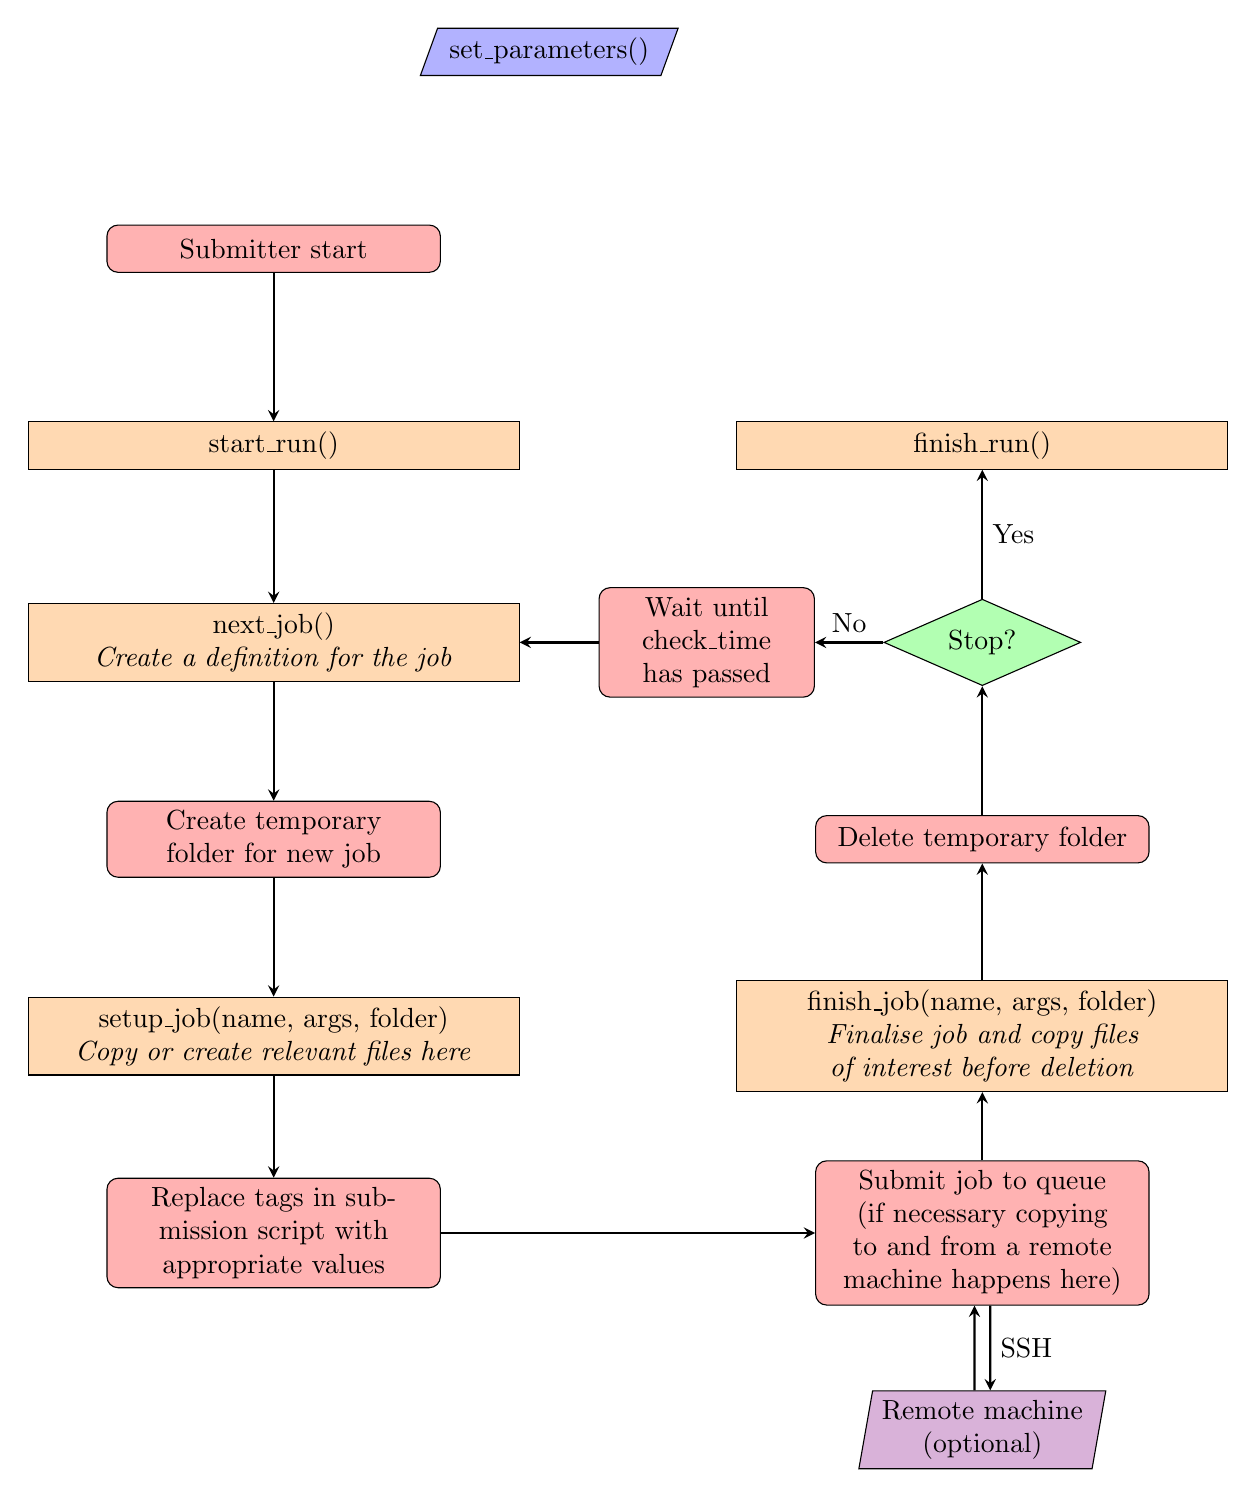
\begin{tikzpicture}[node distance=2.5cm]

\node (in1) [io] {set\_parameters()};
\node (start) [startstop, below of=in1, xshift=-3.5cm] {Submitter start};
\node (startrun) [process, below of=start] {start\_run()};
\node (nextjob) [process, below of=startrun] {next\_job()\\\textit{Create a definition for the job}};
\node (makedir) [startstop, below of=nextjob] {Create temporary folder for new job};
\node (setupjob) [process, below of=makedir] {setup\_job(name, args, folder)\\\textit{Copy or create relevant files here}};
\node (tagscript) [startstop, below of=setupjob] {Replace tags in submission script with appropriate values};
\node (runjob) [startstop, right of=tagscript, xshift=6.5cm] {Submit job to queue (if necessary copying to and from a remote machine happens here)};
\node (finjob) [process, above of=runjob] {finish\_job(name, args, folder)\\\textit{Finalise job and copy files of interest before deletion}};
\node (deldir) [startstop, above of=finjob] {Delete temporary folder};
\node (finished) [decision, above of=deldir] {Stop?};
\node (continue) [startstop, left of=finished, xshift=-1cm, text width=2.5cm] {Wait until check\_time has passed};
\node (finishrun) [process, above of=finished] {finish\_run()};
\node (machine) [machine, below of=runjob] {Remote machine\\
	(optional)};

\draw [arrow] (start) -- (startrun);
\draw [arrow] (startrun) -- (nextjob);
\draw [arrow] (nextjob) -- (makedir);
\draw [arrow] (makedir) -- (setupjob);
\draw [arrow] (setupjob) -- (tagscript);
\draw [arrow] (tagscript) -- (runjob);
\draw [arrow] (runjob) -- (finjob);
\draw [arrow] (finjob) -- (deldir);
\draw [arrow] (deldir) -- (finished);
\draw [arrow] (finished) -- node [anchor=south] {No} (continue);
\draw [arrow] (continue) -- (nextjob);
\draw [arrow] (finished) -- node [anchor=west] {Yes} (finishrun);
\draw [arrow, transform canvas={xshift=0.1cm}] (runjob) -- node [anchor=west] {SSH} (machine);
\draw [arrow, transform canvas={xshift=-0.1cm}] (machine) -- (runjob);

\end{tikzpicture}

\begin{itemize}
	\item \lstinline|set_parameters(**kwargs)| - Must be executed by hand by the user after creating the Submitter instance. Can be overridden and have any interface. Since the \lstinline|__init__| method should \textit{not} be altered, this method provides a way for the user to feed class-specific parameters to any derived Submitter types. 
	\item \lstinline|start_run()| - Executed at the beginning of a run. Here any tasks that are preparatory to initialising the entire run should be accomplished. By default does nothing.
	\item \lstinline|next_job()| - Executed whenever the Submitter has a free slot to start a new job. Should return a definition for said job in the form of a dictionary containing a \lstinline|name| (in the form of a string) and some \lstinline|args| in the form of a dictionary: by default returns \lstinline|{`name': `default_job', `args': {}}|.
	\item \lstinline|setup_job(name, args, folder)| - Executed immediately after \lstinline|next_job()| and the creation of a temporary folder to contain its files. Must perform any operations required to set up the input for the upcoming calculations. For example, \lstinline|next_job| could return a Python object defining an atomic structure on which the calculation ought to be performed; \lstinline|setup_job| is where the input files to which said structure is written should be created and saved in the path defined by \lstinline|folder|.
	\item \lstinline|finish_job(name, args, folder)| - Executed once the job has been run and the output files are in \lstinline|folder| (if the job has been run on a remote machine, at this point the files will have been downloaded back to the local file system). At this point any post-processing should be done and any output files of relevance should be \textit{copied to a persistent folder}. This is especially important as after this step the temporary folder will be deleted.
	\item \lstinline|finish_run()| - Executed at the end of the run, takes care of clean up. If any files need to be closed or resources deallocated this is the place to do it. By default does nothing.
	\item \lstinline|save_state()| - Only executed when the Submitter is initialised with the argument \lstinline|continuation=True|. This allows the Submitter to be stopped (or in case of accidents, crash) and store its current state in order for it to be restarted manually at a later time. By default the submitter only stores the list of the currently running jobs so that it can get back to monitoring them; however, here the user can define any additional data they want to be stored as well, as long as it can be `pickled' \footnote{For more information on the process of serialisation, or `pickling', in Python, see: https://docs.python.org/2.7/library/pickle.html}. This data must be returned as members inside a dictionary. This method \textit{must} return a dictionary, even if empty. The file is saved as \lstinline|<name>.pkl|, where \lstinline|<name>| is the `name' argument passed to the Submitter's constructor.
	\item \lstinline|load_state(loaded_data)| - Only executed when the Submitter is initialised with the argument \lstinline|continuation=True| and a previously saved state file is found. Receives as argument a dictionary containing the saved data; this should be in the same format as the one returned by \lstinline|save_state|. In general it should perform the same operations in reverse, restoring the Submitter to its original state.
\end{itemize}

\section{Writing a tagged submission script}

When submitting a job to a queueing system, one needs to do so in the form of a script, which usually contains the desired commands as well as a number of comments functioning as parameters for the queueing system itself. In the simplest case, this script could be limited to an executable (the program we need to run) and the name of its input file. When creating jobs with a Submitter, this script will be ran from within the folder in which the input files have been created with \lstinline|setup_job|; however, it is reasonable to imagine that these might have different file names or parameters from job to job. To account for that, when one creates a submitter, a script is passed to in which any word that is supposed to change is replaced by a tag surrounded by angle brackets. The main purpose for this is to use the argument \lstinline|name|; the same can be done with any element appearing in the \lstinline|args| dictionary returned as part of the output of \lstinline|next_job|. So for example

\begin{lstlisting}[language=bash]
echo "<sentence>" > <name>.txt
\end{lstlisting}

for a job defined as 

\begin{lstlisting}[language=python]
{'name': 'hello', 
 'args': {'sentence': 
          'Hello World!'}
}
\end{lstlisting}

would produce a file named \lstinline|hello.txt| containing the sentence ``Hello World!".

\section{Creating a Submitter instance}\label{subm_instance}

Given that one has created and specified a derived Submitter class and a properly tagged submission script, it is then necessary to create a file that defines an instance of the Submitter itself. Assuming that we already imported the definition of the new class, the basic template for such a file will be

\begin{lstlisting}[language=python]
from soprano.hpc.submitter import QueueInterface

# Other interfaces supported are LSF and PBS,
# plus you can define your own.
myQ = QueueInterface.GridEngine() 
# Here we load the script
myScr = open('tagged_script.sh').read()

mySub = MySubmitter('test_submitter', myQ, myScr)
mySub.set_parameters(...) # Any parameters needed...
\end{lstlisting}

The constructor for a Submitter takes a number of optional parameters beyond the three obligatory ones (name, queue interface and script). They can all be found in the documentation but for convenience here's a rundown:

\begin{itemize}
	\item \lstinline|max_jobs (Optional[int])| - maximum number of jobs to submit at a given time. When this number of job has been submitted to the queue, the Submitter stops and waits until one of them is complete. Default is 4.
	\item \lstinline|check_time (Optional[float])| - time in seconds between consecutive checks for the queue status and attempts to submit new jobs. Default is 10.
	\item \lstinline|max_time (Optional[float])| - time in seconds the Submitter will run for before shutting down. If set to zero the thread won't stop until killed with Submitter.stop.
	\item \lstinline|temp_folder (Optional[str])| - where to store the temporary folders for the calculations. By default it's the current folder.
	\item \lstinline|remote_workdir (Optional[str])| - if present, uses a directory on a remote machine by logging in via SSH. Must be in the format \lstinline|<host>:<path/to/directory>| (without the angle brackets, replace host name and directory suitably; the directory must already exist). Host must be defined in the user's \lstinline|~/.ssh/config file| - check the docs for RemoteTarget for more information. It is possible to omit the colon and directory, that will use the home directory of the given folder; that is HEAVILY DISCOURAGED though. Best practice would be to create an empty directory on the remote machine and use that, to avoid accidental overwriting/deleting of important files.
	\item \lstinline|remote_getfiles (Optional[list(str)])| - list of files to be downloaded from the remote copy of the job's temporary directory. By default, all of them. Can be a list using specific names or wildcards. Filenames can also use the placeholder {name} to signify the job name, as well as any other element from the arguments.
	\item \lstinline|ssh_timeout (Optional[float])| - connection timeout in seconds. Default is 1.
	\item \lstinline|continuation (Optional[bool])| - if True, when the Submitter is stopped it will not terminate the current jobs; rather, it will store the list of ongoing jobs in a pickle file. If the submitter is ran again from the same folder then it will "pick up from where it left" and try recovering those jobs, then restart. If one wishes for additional values to be saved and restored, the \lstinline|save_state| and \lstinline|load_state| methods need to be defined.
\end{itemize}

\section{Launching a Submitter}

Finally, once everything in place, it is possible to launch the Submitter. This is done by running the command \lstinline|soprano_submitter.py|. The syntax is described as follows:

\begin{lstlisting}
soprano_submitter.py [-h] [-n N] [-nohup] action submitter_file
\end{lstlisting}

where \lstinline|submitter_file| is the name of the file in which the \textit{instance} of the Submitter was created (as described in \ref{subm_instance}) and \lstinline|action| can be one of \lstinline|start|, \lstinline|stop| or \lstinline|list|. The previous two are pretty self-explanatory; the third lists which Submitters, among the ones defined in the given file, are running, and how long they have been. The additional options work as follows:

\begin{itemize}
	\item \lstinline|-h| - display the help message
	\item \lstinline|-n N| - launch the submitter of name N. This must be used when multiple Submitters are instanced in \lstinline|submitter_file|. The name must be the name of the variable (so for example in the example in \ref{subm_instance}, that would be \lstinline|mySub|)
	\item \lstinline|-nohup| - put the Submitter thread in `no hangup' mode, meaning that it will keep running even if one closes the terminal session from which it was launched. This is mainly for the case in which a Submitter was launched on a machine to which we connect remotely via \lstinline|ssh|.
\end{itemize}

When a Submitter is started it runs in the background of a shell session until \lstinline|max_time| seconds have passed or it is explicitly stopped. When stopped, if \lstinline|continuation=True| wasn't set, it kills all still ongoing jobs and deletes all the temporary folders; otherwise it leaves everything running and stores a pickled file with the pattern \lstinline|<submitter_name>.pkl| in the current folder from which it can pick back up. Deleting the file in question is equivalent to resetting the run. During and at the end of a run, a log file called \lstinline|<submitter_name>.log| is available containing messages detailing the workings of the Submitter. When defining a new Submitter class, one can use the method \lstinline[language=python]|self.log('Message')| inside it to write to this log file additional lines.



\end{document}          
